\documentclass[12pt, a4paper]{article}

\usepackage{fancyhdr}
\usepackage[left=4cm, right=4cm, top=4cm, bottom=4cm]{geometry}
\usepackage[utf8]{inputenc}
\usepackage[table]{xcolor}
\usepackage{hyperref}
\usepackage{amsmath}
\usepackage{enumitem}
\usepackage{graphicx}
\usepackage{booktabs}
\usepackage{subcaption}
\usepackage[justification=centering]{caption}
\usepackage{xepersian}

\DeclareMathOperator*{\argmax}{argmax}
\DeclareMathOperator*{\argmin}{argmin}
\newcolumntype{L}{>{$}l<{$}} % math-mode version of "l" column type

\newcommand{\coursetitle}{شبکه‌های عصبی}
\newcommand{\doctitle}{تمرین دوم}
\newcommand{\name}{محمدرضا غفرانی}
\newcommand{\studentno}{400131076}
\newcommand{\todaydate}{\today}

\settextfont{XB Kayhan}
\setlatintextfont{Times Newer Roman}

\pagestyle{fancy}
\lhead{\textbf{\doctitle}}
\chead{\name}
\rhead{\todaydate}

\begin{document}

\begin{flushleft}
    \name \\
    \studentno \\
    \todaydate
\end{flushleft}

\begin{center}
    \huge
    \textbf{\coursetitle}
    \break
    \large
    \doctitle
\end{center}

% suppress the fancy header on the first page only
\thispagestyle{plain}

\section*{سوال یک}

\subsection*{شبکه \lr{LeNet-5}}

این شبکه عصبی از ۵ لایه تشکیل شده است. سه لایه‌ کانولوشنی بوده و باقی لایه‌ها
از نوع \lr{fully connected} هستند. در ادامه ساختار هر یک از این لایه‌های این شبکه عصبی توضیح داده می‌شود.

\begin{enumerate}
    \item لایه کانولوشنی: این لایه کانولوشنی دارای 6 فیلتر با ابعاد $5 \times 5$ بوده و با
    اندازه قدم یک بر روی تصویر ورودی اعمال می‌شود. تابع فعال‌ساز این لایه $\tanh$ است. با توجه به این که
    این لایه ۶ فیلتر را بر روی تصویر ورودی اعمال می‌کند، بنابراین این لایه تصویر تک کاناله ورودی را به
    ۶ کانال مجزا نگاشت می‌کند.
    \begin{enumerate}
        \item \lr{Pooling}: در این قسمت یک فیلتر $2 \times 2$ روی خروجی لایه اعمال می‌شود. فیلتر اعمال شده
        از نوع \lr{average-pooling} بوده و تعداد کانال‌های ورودی را تغییر نمی‌دهد. اما ابعاد هر ورودی دریافتی
        را نصف می‌کند.
    \end{enumerate}
    \item لایه کانولوشنی: در این لایه ۱۶ فیلتر با ابعاد $5 \times 5$ و اندازه قدم یک به خروجی‌های لایه قبلی اعمال می‌شود.
    تابع فعال این لایه نیز $\tanh$ است.
    \begin{enumerate}
        \item \lr{Pooling}: در این قسمت نیز یک فیلتر $2 \times 2$ بر روی خروجی لایه قبلی اعمال شده و ابعاد خروجی‌های
        لایه قبلی را نصف می‌کند.
    \end{enumerate}
    \item لایه کانولوشنی: این لایه با اعمال ۱۲۰ فیلتر با ابعاد $5 \times 5$ ابعاد خروجی تمام کانال‌ها را به یک بعد می‌رساند.
    تابع فعال‌ساز این لایه نیز مشابه لایه‌های قبلی $\tanh$ است.
    \item لایه \lr{fully-connected}: این لایه‌ خروجی لایه قبلی را گرفته و عمل دسته‌بندی را آغاز می‌کند. همان‌طور که از نام این
    لایه مشخص است، هر گره این لایه به تمامی گره‌های لایه بعدی متصل است.
    \item لایه \lr{fully-connected}: عملکرد این لایه نیز مشابه لایه \lr{fully-connected} قبلی است. معمولا خروجی این لایه
    را به یک لایه \lr{softmax} می‌دهند تا خروجی نهایی مدل مشخص شود.
\end{enumerate}

در شکل \ref{lenet} ساختار این شبکه در هنگام اعمال بر روی یک تصویر سیاه‌ و سفید با ابعاد $32 \times 32$ مشاهده می‌شود.

\begin{figure}[h]
    \centering
    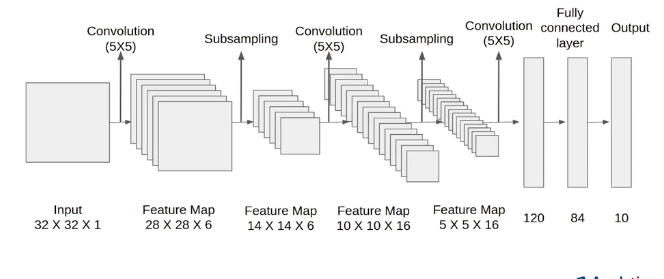
\includegraphics[width=0.8\linewidth]{images/lenet.png}
    \caption{نمونه‌ای از شبکه عصبی \lr{LeNet}}
    \label{lenet}
\end{figure}

\subsection*{شبکه \lr{Inception}}

با افزایش تعداد لایه‌های کانولوشنی احتمال بیش‌برازش مدل روی داده‌های آموزشی بیشتر می‌شود.
برای رفع این مشکل در نسخه اول شبکه \lr{Inception} چند فیلتر کانولوشنی در یک سطح از شبکه
استفاده شد. این ایده باعث شد مدل نسبت به مدل‌های پیشین عملکرد بهتری داشته باشد. از طرف دیگر در این مدل
به جهت کاهش ابعاد و همچنین افزایش سرعت به هر لایه یک فیلتر کانولوشنی $1 \times 1$ اضافه شده است.
در شکل \ref{inceptionv1_convolution} نوآوری‌های انجام شده این مدل نشان داده شده است.

\begin{figure}[h]
    \begin{subfigure}{0.45\linewidth}
        \centering
        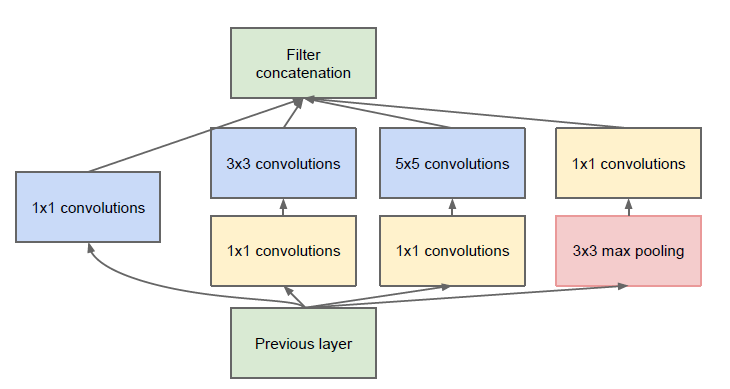
\includegraphics[width=0.8\linewidth]{images/inception/1by1.png}
        \caption{شیوه قرارگیری فیلترها با اضافه‌کردن فیلتر $1 \times 1$}
    \end{subfigure}
    \hfill
    \begin{subfigure}{0.45\linewidth}
        \centering
        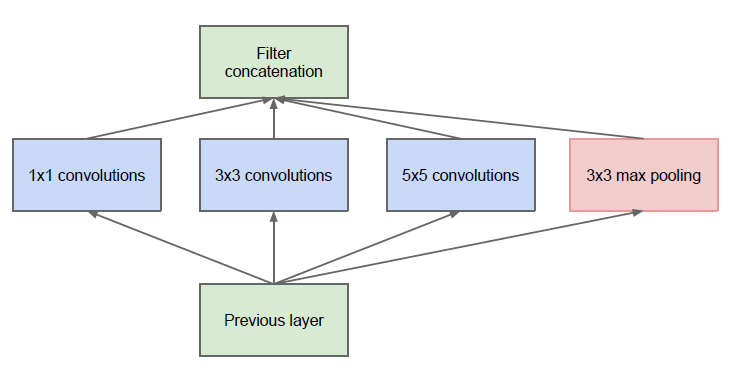
\includegraphics[width=0.8\linewidth]{images/inception/before_1by1.png}
        \caption{شیوه قرارگیری فیلترها قبل از اضافه‌کردن فیلتر $1 \times 1$}
    \end{subfigure}
    \caption{}
    \label{inceptionv1_convolution}
\end{figure}

در مدل \lr{Inception v3} ایده‌های بالا به همراه دیگر ایده‌هایی که در ادامه توضیح داده می‌شود،
برای بهبود عملکرد مدل به کار گرفته شده است.

\begin{itemize}
    \item \textbf{تبدیل فیلتر‌های با ابعاد بالا به چند فیلتر با ابعاد کوچک‌تر} کاهش بعد یکی از ویژگی‌های مثبت
    مدل \lr{Inception v1} بود. نسخه سوم این مدل هم این ویژگی خوب را به ارث برد و حتی آن را
    بهبود داد. در تصویر \ref{improved_conv} ایده نسخه سوم مدل مشاهده می‌شود. در شبکه \lr{Inception v3}
    مطابق شکل فیلتر‌های با ابعاد $5 \times 5$ به دو فیلتر با ابعاد $3 \times 3$ تبدیل می‌شود. این تبدیل باعث کاهش
    تعداد پارامتر‌های مدل و افزایش سرعت مدل می‌شود. در شکل \ref{two3_img} نمونه‌ای از عملکرد دو فیلتر $3 \times 3$
    که به صورت متوالی قرار داده شده است، آورده شده است.

    \begin{figure}[h]
        \begin{subfigure}{0.45\linewidth}
            \centering
            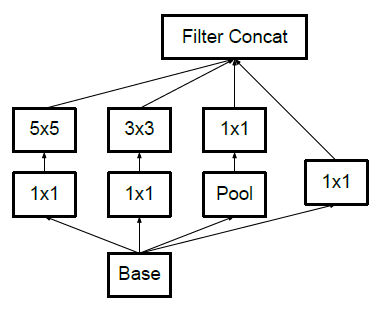
\includegraphics[width=0.8\linewidth]{images/inception/inceptionv1_conv.png}
            \caption{معماری فیلتر‌های مدل \lr{Inception v1}}
            \label{improved_conv_inceptionv1}
        \end{subfigure}
        \hfill
        \begin{subfigure}{0.45\linewidth}
            \centering
            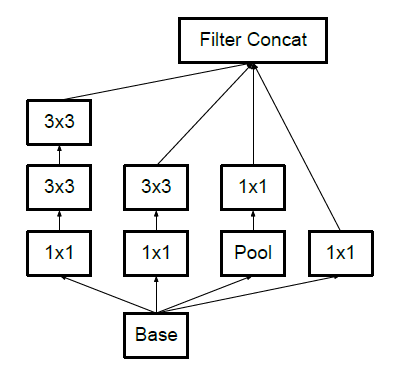
\includegraphics[width=0.8\linewidth]{images/inception/inceptionv3_conv.png}
            \caption{معماری فیلتر‌های مدل \lr{Inception v3}}
            \label{improved_conv_inceptionv3}
        \end{subfigure}
        \caption{شیوه کاهش ابعاد فیلتر‌های کانولوشنی در مدل \lr{inceptionv3}}
        \label{improved_conv}
    \end{figure}

    \begin{figure}[h]
        \centering
        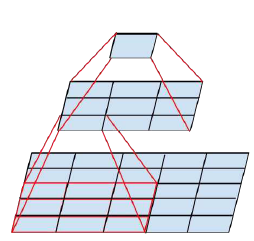
\includegraphics[width=0.3\linewidth]{images/inception/two3_img.png}
        \caption{}
        \label{two3_img}
    \end{figure}

    \item \textbf{تبدیل فیلتر‌ها به فیلتر‌های نامتقارن} با توجه به مزیت‌هایی که کاهش ابعاد فیلتر‌ها در کنار
    افزایش تعداد آن‌ها برای ما به همراه داشته است به نظر می‌رسد که ایده خوبی باشد که فیلتر‌های $3 \times 3$ نیز به
    فیلتر‌های $2 \times 2$ تبدیل شود. اما این تبدیل کاهش بعد چندانی نداشته و مزیتی ایجاد نمی‌کند. روش دیگر آن است که
    ابعاد فیلتر‌ها را نامتقارن در نظر بگیریم. این ایده در شکل \ref{asymetric_fact} دیده می‌شود. با این کار
    پارامتر‌های مدل به شکل چشم‌گیری کاهش می‌یابد. در شکل \ref{asymetric_example} نمونه‌ای از اعمال این ایده
    بر روی شکل \ref{improved_conv_inceptionv3} دیده می‌شود.

    \begin{figure}[h]
        \begin{subfigure}{0.45\linewidth}
            \centering
            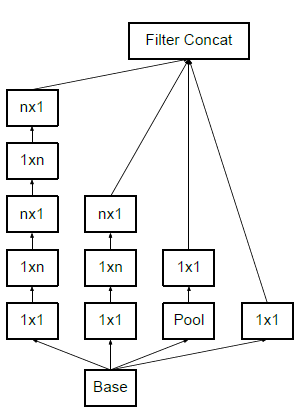
\includegraphics[scale=0.4]{images/inception/asymetric.png}
            \caption{}
            \label{asymetric_fact}
        \end{subfigure}
        \begin{subfigure}{0.45\linewidth}
            \centering
            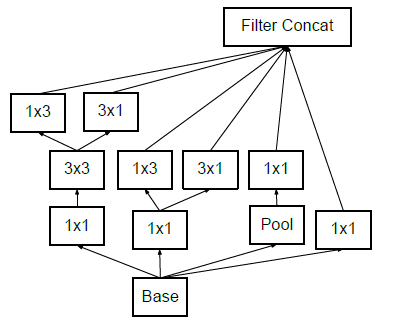
\includegraphics[scale=0.4]{images/inception/asymetric_example.png}
            \caption{}
            \label{asymetric_example}
        \end{subfigure}
        \caption{شیوه فاکتورکردن نامتقارن و مثالی از آن}
    \end{figure}

    \item \textbf{استفاده از دسته‌بند‌های کمکی} هدف از استفاده از دسته‌بندهای کمکی افزایش همگرایی مدل‌های
    عصبی عمیق است. این دسته‌بندها بیشتر به منظور جلوگیری از مشکل \lr{vanishing gradient} استفاده می‌شوند.
    در شبکه \lr{Inception} این دسته‌بند در گام‌های اولیه یادگیری بهبودی ایجاد نمی‌کند. اما با نزدیک شدن به گام‌های
    نهایی، عملکرد شبکه‌ای که از دسته‌بند کمکی استفاده کرده است بسیار بهتر از شبکه بدون دسته‌بند است.
    به عبارتی دیگر این دسته‌بندی کمکی نظیر یک هموارساز عمل کرده و عملکرد مدل را بهبود می‌دهد.

    \item \textbf{کاهش بهینه ابعاد(\lr{Efficient Grid Size Reduction})} در شبکه \lr{Inception v3} بر خلاف
    روال معمول که از دو تابع \lr{max pooling} و \lr{average pooling} برای کاهش ابعاد مدل استفاده می‌شود.
    از دو ساختار موجود در شکل \ref{reducer} برای کاهش ابعاد استفاده می‌شود.

    \begin{figure}[h]
        \centering
        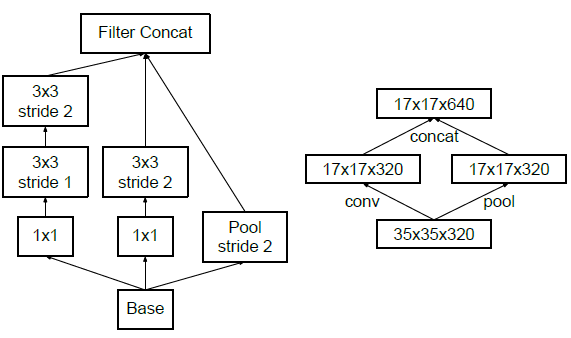
\includegraphics[width=0.7\linewidth]{images/inception/reducer2.png}
        \caption{شبکه‌هایی که برای کاهش بعد در مدل \lr{Inception v3} استفاده می‌شود.}
        \label{reducer}
    \end{figure}

\end{itemize}

شکل کلی مدل \lr{Inception v3} در شکل \ref{inception} آورده شده است. همان‌طور که مشاهده می‌شود معماری مدل
\lr{LeNet} نسبت به مدل \lr{Incpetion} بسیار کوچک‌تر است. مدل \lr{Inception} تعداد لایه‌های بیشتری داشته
و در نتیجه مدل عمیق‌تری است. عمیق‌تر بودن باعث شده است که به راحتی بتواند الگوی داده‌ها را کشف کرده و
به نتایج بسیار خوبی برسد. البته عمیق بودن هم مزیت و هم عیب مدل محسوب می‌شود. به دلیل عمیق بودن ممکن است
روی داده‌های آموزشی بیش‌برازش شود، در نتیجه راهکار‌های فراوانی را هم برای جلوگیری از وقوع مشکلاتی نظیر
\lr{vanishing problem} و بیش‌برازش پیاده‌سازی کرده است. به خاطر همین عمیق بودن به زمان بیشتری برای آموزش
مدل نیاز داشته و در هنگام تست نیز مدت زمان بیشتری برای پاسخ دادن به داده ورودی نیاز دارد. اما در حالت
کلی از آن جا که عملکرد بهتری نسبت به مدل \lr{LeNet} دارد در نتیجه نسبت به آن بهتر است.

\begin{figure}[h]
    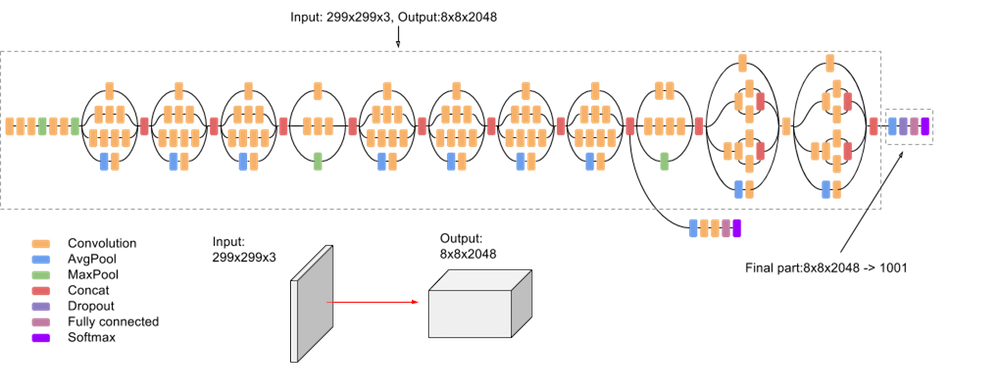
\includegraphics[width=0.8\linewidth]{images/inception/inception}
    \caption{معماری کلی شبکه \lr{Inception}}
    \label{inception}
\end{figure}

\pagebreak

\section*{سوال دو}

شبکه \lr{LeNet} انتظار دارد ورودی یک تصویر تک‌کاناله با ابعاد $32 \times 32$ باشد. اما تصاویر مجموعه داده ما
$500 \times 500$ بوده و سه کاناله هستند. به همین دلیل با انجام پیش‌پردازش روی داده‌ها آن‌ها را به تصاویر
سیاه‌وسفید تبدیل کرده و اندازه تصاویر را نیز به $32 \times 32$ تبدیل می‌کنیم.

شبکه \lr{LeNet} از آن جا که برای شناسایی رقم‌های دست‌نویس ارائه شده است،
دارای ۱۰ نود در لایه خروجی است. اما در این جا می‌خواهیم داده‌ها را به سه کلاس تقسیم کنیم؛ بنابراین لایه خروجی شبکه
را تغییر داده و تعداد نود‌های خروجی آن را به ۳ کاهش می‌دهیم. به جز این موارد پیش‌پردازش یا تغییر دیگری
در ساختار مدل انجام نشده است. عملکرد مدل در این حالت در جدول \ref{lenet_base_result} آورده شده است.

\begin{latin}
\begin{table}[h]
    \centering
    \caption{\rl{جدول عملکرد شبکه \lr{LeNet} در حالت پایه}}
    \label{lenet_base_result}
    \begin{tabular}{l|l||l|l||l|l}
        \multicolumn{2}{c||}{train} & \multicolumn{2}{c||}{validation} & \multicolumn{2}{c}{test} \\ \hline
        loss & acc & loss & acc & loss & acc\\ \hline
        0.84 & 0.62 & 0.95 & 0.6 & 0.96 & 0.55
    \end{tabular}
\end{table}
\end{latin}

\subsection*{قسمت الف}

در ادامه تاثیر افزودن هر یک از لایه‌های منظم‌ساز بررسی می‌شود.

\begin{itemize}
    \item \textbf{منظم‌ساز \lr{L1}}: در هنگام منظم‌سازی با استفاده از پارامتر \lr{L1} هنگامی که پارامتر
    منظم‌سازی عدد کوچکی نظیر $10^{-6}$ است عملکرد مدل اندکی بهتر می‌شود.
    اما اگر مقادیر بزرگی نظیر $0.1$ را برای تنظیم مدل در نظر بگیریم، عملکرد مدل هم در داده‌های
    ارزیابی و هم داده‌های آموزش افت می‌کند. (جدول \ref{lenet_l1_reg})
    \begin{latin}
    \begin{table}[h]
        \centering
        \caption{\rl{عملکرد شبکه \lr{LeNet} با منظم‌ساز \lr{L1}}}
        \label{lenet_l1_reg}
        \begin{tabular}{l|l|l||l|l||l|l}
            & \multicolumn{2}{c||}{train} & \multicolumn{2}{c||}{validation} & \multicolumn{2}{c}{test} \\ \hline
            L1 value & loss & acc & loss & acc & loss & acc\\ \hline
            $10^{-6}$ & 0.77 & 0.66 & 0.91 & 0.59 & 0.88 & 0.59\\
            $0.1$ & 1.32 & 0.34 & 1.32 & 0.34 & 1.32 & 0.34
        \end{tabular}
    \end{table}
    \end{latin}
    \item \textbf{منظم‌ساز \lr{L2}}: نتایج حاصل شده در هنگام استفاده از این منظم‌ساز بسیار شبیه نتایج حاصل شده در حالت استفاده
    از منظم‌ساز \lr{L1} بوده و تفاوت فاحشی بین آن‌ها نیست.
    این شباهت قابل توجیه است. فرمول هموار‌سازی \lr{L2} بسیار شبیه \lr{L1} است
    بنابراین منطقیست که عملکرد این دو تابع هموار‌ساز شبیه یکدیگر باشند. (جدول \ref{lenet_l2_reg})
    \begin{latin}
    \begin{table}[h]
        \centering
        \caption{\rl{عملکرد شبکه \lr{LeNet} با منظم‌ساز \lr{L2}}}
        \label{lenet_l2_reg}
        \begin{tabular}{l|l|l||l|l||l|l}
            & \multicolumn{2}{c||}{train} & \multicolumn{2}{c||}{validation} & \multicolumn{2}{c}{test} \\ \hline
            L2 value & loss & acc & loss & acc & loss & acc\\ \hline
            $10^{-6}$ & 0.79 & 0.59 & 0.95 & 0.59 & 0.92 & 0.55 \\
            $0.1$ & 1.19 & 0.63 & 1.28 & 0.56 & 1.24 & 0.57
        \end{tabular}
    \end{table}
    \end{latin}

    \item \textbf{منظم‌ساز \lr{DropOut}}: تاثیر وجود این لایه همانند تاثیر وجود منظم‌ساز‌های \lr{L1} و \lr{L2} است. بدین
    معنی که هنگامی که مقدار نرخ \lr{dropout} مدل کم است (مثلا در حد $10^{-2}$یا $10^{-4}$) عملکرد مدل در داده‌های ارزیابی
    اندکی بهتر از حالت پایه می‌شود. با زیاد کردن نرخ \lr{dropout} نیز (در حد $0.7$) مدل نمی‌تواند روی داده‌های ارزیابی و آموزشی به نتایج خوبی برسد.
    \begin{latin}
    \begin{table}[h]
        \centering
        \caption{\rl{عملکرد شبکه \lr{LeNet} با منظم‌ساز \lr{Dropout}}}
        \label{lenet_dropout_reg}
        \begin{tabular}{l|l|l||l|l||l|l}
            & \multicolumn{2}{c||}{train} & \multicolumn{2}{c||}{validation} & \multicolumn{2}{c}{test}\\ \hline
            dropout value & loss & acc & loss & acc & loss & acc\\ \hline
            $10^{-4}$ & 0.78 & 0.66 & 0.94 & 0.6 & 0.95 & 0.5\\
            $0.7$ & 0.97 & 0.54 & 0.98 & 0.54 & 0.99 & 0.48
        \end{tabular}
    \end{table}
    \end{latin}

\end{itemize}

با توجه به یکسان بودن نتایج و عملکرد تقریبا یکسان مدل با اضافه کردن هموار‌سازی‌های مختلف نتایج حاصل شده را یکجا توجیه می‌کنیم.
هدف ما از اضافه‌کردن هموار‌سازی‌های مختلف به مدل جلوگیری از بیش‌برازش مدل‌ بر روی داده آموزشی و رسیدن به نتیجه بهتر در
داده‌های ارزیابی بود. در تمامی تکنیک‌های هموار‌سازی استفاده شده، هنگامی که پارامتر هموار‌سازی عدد کوچکی بود همان‌طور که دیدیم
عملکرد مدل در داده‌ها اندکی بهتر می‌شود. این مورد نشان می‌دهد که
به ازای اضافه‌کردن این هموار‌سازی‌ها مدل دست از بیش‌برازش روی داده‌های آموزشی برداشته که در نتیجه به نتایج بهتر روی داده‌های
ارزیابی رسیده است. اما هنگامی که پارامتر هموارسازی را بیشتر می‌کردیم،‌ عملکرد مدل هم در داده‌های ارزیابی و هم در داده‌های
آموزشی بدتر می‌شد که نشان می‌داد مدل به دلیل وجود لایه هموار‌سازی نمی‌تواند دانش چندانی در رابطه با داده‌ها بیاموزد.

\subsection*{قسمت ب}

با توجه به جدول \ref{impact_of_filter_count_on_lenet} به صورت کلی می‌توان گفت که افزایش تعداد فیلتر‌های کانولوشنی
باعث بهترشدن عملکرد مدل می‌شود. برای مثال در حالتی که تعداد فیلتر‌ها برابر $(100,100,20)$ است، مدل توانسته است
صحت خوبی را در داده‌های آزمون داده با کم‌کردن نرخ \lr{loss} ارائه دهد. البته این افزایش عملکرد بدون هزینه نیز نبوده و
مدل به مدت زمان بیشتری نیاز دارد تا هر گام یادگیری را طی کند. همچنین با افزایش لایه‌های کانولوشنی به دلیل
آزادی عملکرد بیشتر، استعداد مدل برای بیش‌برازش روی داده‌های آموزشی بیشتر می‌شود. بنابراین برای آن که هر مدل
بهترین عملکرد خود را داشته باشد، از یک \lr{EarlyCallback} با حداکثر تعداد صبر ۳ واحد استفاده کرده‌ایم.
اگر نرخ \lr{loss} در داده اعتبارسنجی در طی سه گام متوالی کاهش نیابد، حداکثر تعداد گام برای آموزش مدل
برابر ۲۰ است.

\begin{latin}
\begin{table}[h]
    \centering
    \caption{\rl{جدول بررسی تاثیر تعداد فیلتر در عملکرد شبکه \lr{LeNet}}}
    \label{impact_of_filter_count_on_lenet}
    \begin{tabular}{l||l|l||l|l||l|l}
        & \multicolumn{2}{c||}{train} & \multicolumn{2}{c||}{validation} & \multicolumn{2}{c}{test}\\ \hline
        \# of filter & loss & acc & loss & acc & loss & acc \\ \hline
        (1,1,1) & 1.1 & 0.33 & 1.1 & 0.33 & 1.1 & 0.34 \\ \hline
        (3,3,2) & 1 & 0.49 & 1.02 & 0.47 & 1.01 & 0.48 \\ \hline
        (20,10,5) & 0.86 & 0.6 & 0.97 & 0.49 & 0.92 & 0.54 \\ \hline
        (50,40,30) & 0.53 & 0.8 & 0.88 & 0.62 & 0.84 & 0.61\\ \hline
        (100,100,20) & 0.4 & 0.88 & 0.88 & 0.61 & 0.82 & 0.62
    \end{tabular}
\end{table}
\end{latin}

\subsection*{قسمت ج}

با توجه به نتایج که در جدول \ref{impact_of_filter_size_on_lenet} آورده شده است، با بیشترکردن ابعاد فیلتر‌های کانولوشن
صحت عملکرد مدل کاهش می‌یابد. این اتفاق را می‌توان این گونه توجیه کرد که هنگامی که ابعاد فیلتر بزرگ است
نمی‌تواند ویژگی‌های کلی مدل را از تصویر استخراج کند، چرا که اندازه تصویر $32 \times 32$ بوده و در نتیجه
با اعمال یک فیلتر $16 \times 16$ در لایه اول ویژگی‌های حاصل شده بسیار کلی می‌شود، که در لایه‌های بعدی با اعمال
فیلتر‌های کوچک‌تر نیز ویژگی‌ها استخراج نمی‌شود. نکته بعدی که وجود دارد محل اعمال این فیلتر است برای مثال هنگامی که
در لایه اول یک فیلتر $5 \times 5$ و در لایه بعدی یک فیلتر $3 \times 3$ اعمال می‌کنیم نتایج بسیار بهتری نسبت به حالتی که
فیلتر $3 \times 3$ در لایه اول است می‌گیریم.

از دیگر پیامد‌های افزایش ابعاد فیلتر‌ها می‌توان به افزایش تعداد پارامتر‌های مدل اشاره کرد. با افزایش تعداد پارامتر‌ها
نیاز به داده بیشتری دارد تا بتواند الگوی کلی داده‌ها را به خوبی پیدا کرده و مقدار بهینه هر پارامتر را به دست آورد.

در این حالت برای آن که تمامی مدل‌ها به بهترین عملکرد خود دست یابند، یک \lr{EarlyCallback} با مشخصات توضیح داده شده
در قسمت قبل آورده شده است.

\begin{latin}
\begin{table}[h]
    \centering
    \caption{\rl{جدول بررسی تاثیر اندازه فیلتر در عملکرد شبکه \lr{LeNet}}}
    \label{impact_of_filter_size_on_lenet}
    \begin{tabular}{l||l|l||l|l||l|l}
        & \multicolumn{2}{c||}{train} & \multicolumn{2}{c||}{validation} & \multicolumn{2}{c}{test}\\ \hline
        size of filter & loss & acc & loss & acc & loss & acc \\ \hline
        (16, 7, 1) & 1.05 & 0.43 & 1.09 & 0.38 & 1.09 & 0.43 \\ \hline
        (14, 5, 2) & 0.97 & 0.43 & 1.04 & 0.47 & 1.08 & 0.43 \\ \hline
        (8, 5, 2) & 0.8 & 0.66 & 0.99 & 0.59 & 0.93 & 0.56 \\ \hline
        (5, 3, 2) & 0.81 & 0.64 & 0.98 & 0.53 & 0.92 & 0.59 \\ \hline
        (3, 5, 2) & 0.8 & 0.64 & 0.98 & 0.48 & 1.07 & 0.45 \\ \hline
    \end{tabular}
\end{table}
\end{latin}

\pagebreak

\section*{سوال سه}

در فرآیند انتقال یادگیری ابتدا مدلی بر پایه مجموعه داده برزگ ساخته می‌شود. در این مرحله مدل دانش خوبی از
کلیات مسئله دارد اما نمی‌تواند در یک وظیفه خاص به خوبی عمل کند. تکنیک‌های انتقال یادگیری به منظور بهتر کردن
عملکرد مدل در حوزه‌های خاص و یا انتقال آموخته‌های  مدل به حوزه‌های مشابه استفاده می‌شود. از تکنیک‌های این دانش
معمولا در دو سناریو استفاده می‌شود.

\begin{itemize}
    \item هنگامی که تعداد داده در دسترس در حوزه مقصد محدود است. در این حالت با تنظیم مدل آموزش دیده در داده‌های
    حجیم با داده‌های حوزه مقصد می‌توان به نتایج قابل قبولی رسید.
    \item سناریو دیگر هنگامی است که می‌خواهیم برای حوزه مدنظر مدلی را به سرعت ارائه دهیم. در این حالت
    به جای آن که مدل را از پایه روی تمامی داده‌ها آموزش دهیم، تلاش می‌کنیم با تغییرات جزئی در مدل حجیم،
    به نتایج خوبی در حوزه مقصد برسیم.
\end{itemize}

با ارائه شبکه‌های عصبی کار‌های فراوانی در زمینه انتقال یادگیری صورت گرفت. معمولا هنگامی که می‌خواهند یک مدل شبکه عصبی را
روی داده‌های دیگری تنظیم کنند، شبکه را اصطلاحا \lr{freeze} کرده و لایه‌های آخری که برای تولید خروجی نهایی هستند را حذف می‌کنند.
وزن‌های آموخته شده برای این لایه‌ها در طی فرآیند تنظیم\LTRfootnote{Fine tune} تغییر نکرده و ثابت می‌ماند. حال لایه‌های
نهایی جدید را اضافه کرده و آموزش را با یادگیری مقادیر وزن این لایه‌ها روی داده‌های حوزه مقصد، پیش می‌برند.
در نهایت با در نظر گرفتن مقادیر بسیار کوچکی برای نرخ یادگیری و آموزش مجدد کل مدل (با \lr{unfreeze}کردن لایه‌ها)
آموزش مدل را نهایی می‌کند.

\section*{سوال چهار}

\subsection*{قسمت الف}

شکل کلی شبکه آموزش دیده برای آموزش مجدد مدل \lr{Inception} در شکل \ref{inception_pretrain} آورده شده است.
همان‌طور که مشاهده می‌شود برای آموزش مجدد مدل یک لایه ورودی به همراه یک لایه \lr{MaxPooling} و یک لایه خروجی از نوع
\lr{Softmax} به مدل اضافه کرده‌ایم. برای مشخص کردن تعداد بهینه لایه‌های فریز شده از آزمون و خطا استفاده می‌کنیم.
بدین شکل که هر بار درصد مشخصی از لایه‌های ابتدایی مدل \lr{inception} فریز شده و باقی لایه‌ها آموزش می‌بینند.

\begin{figure}[h]
    \centering
    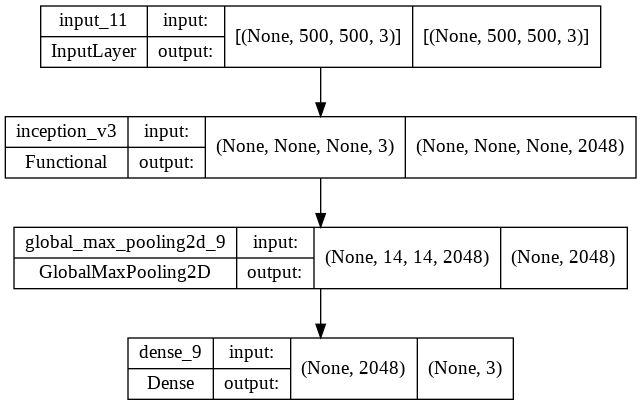
\includegraphics[width=0.8\linewidth]{images/inception.png}
    \caption{شبکه طراحی شده برای آموزش مجدد مدل \lr{Inception}}
    \label{inception_pretrain}
\end{figure}

سعی و خطاهای انجام شده برای آموزش مدل در جدول \ref{frozen_inception} آورده شده است. همچنین لازم به ذکر است که
به دلیل زمان‌بر بودن آموزش مدل تعداد گام آموزش را برابر ۷ در نظر گرفته‌ایم. با توجه به نتایج، مدل به ازای
این تعداد گام فرصت کافی برای آموزش و یافتن مقدار بهینه برای پارامتر‌های خود را داشته است.

در توضیح نتایج باید گفت که مدل هنگامی که بیشتری آزادی عمل را داشته است توانسته به بهترین نتیجه برسد،
اما در ادامه با محدودشدن آزادی عمل مدل، توانایی شبکه ضعیف و ضعیف‌تر شده است تا جایی که عملکرد مدل حتی
از مدل \lr{LeNet} هم ضعیف‌تر شده است. بنا بر این توضیح فاکتور‌های زیر را می‌توان در هنگام افزایش
تعداد لایه‌های فریزشده مدل دخیل دانست.

\begin{itemize}
    \item \textbf{تعداد گام و محاسبات.} مشخص است که هر چه تعداد لایه‌های فریزشده کمتر باشد،
    تعداد پارامتر‌های مدل بیشتر بوده و در نتیجه مدل به مدت زمان و تعداد گام بیشتری برای یافتن بهترین مقدار
    این پارامتر‌ها نیاز دارد.
    \item \textbf{حوزه آموزش مدل ازپیش‌آموزش‌دیده.} اگر مدل ازپیش‌آموزش‌دیده پیش‌تر در حوزه دیگری آموزش دیده باشد که با حوزه مقصد
    تفاوت داشته باشد برای آن که بتواند روی حوزه مقصد به خوبی عمل کند نیاز به آزادی عمل بیشتر و تعداد لایه‌های
    فریزشده کم‌تری دارد تا بتواند پارامتر‌ها را به خوبی در حوزه جدید آموزش دهد. اما اگر حوزه عملکرد مدل
    چندان متفاوت نباشد، می‌توان با فریز کردن تعداد لایه‌های کمتر به دقت‌های خوبی رسید.
\end{itemize}

نکته جالبی که در خصوص \lr{Fine-tune} این شبکه وجود دارد این است که اگر ابتدا بخواهیم تمامی لایه‌های شبکه \lr{Inception}
را فریز کرده و پس از آموزش لایه‌های جدید اضافه شده، بخش‌هایی از مدل ازپیش‌آموزش دیده را \lr{unfreeze} کرده و \lr{Fine-tune}
کنیم مدل نهایی عملکرد ضعیف‌تری خواهد داشت. به همین دلیل ما در هنگام آموزش لایه‌های جدید، بخش‌هایی از مدل \lr{Inception}
را نیز \lr{unfreeze} کرده و آموزش می‌دهیم. نتایج موجود در جدول \ref{frozen_inception} با همین روش حاصل شده‌اند.

\begin{latin}
    \begin{table}[h]
    \centering
    \caption{\rl{درصد لایه‌های فریز شده مدل ازپیش‌آموزش‌دیده}}
    \label{frozen_inception}
    \begin{tabular}{l||l|l||l|l||l|l}
        & \multicolumn{2}{c||}{train} & \multicolumn{2}{c||}{validation} & \multicolumn{2}{c}{test}\\ \hline
        \% of frozen layer & acc & loss & acc & loss & acc & loss \\ \hline
        0 & 1 & 0 & 0.95 & 0.14 & 0.9 & 0.32 \\ \hline
        10 & 1 & 0 & 0.8 & 0.71 & 0.81 & 0.56 \\ \hline
        20 & 1 & 0.02 & 0.66 & 0.9 & 0.67 & 0.86 \\ \hline
        30 & 1 & 0.01 & 0.62 & 1.28 & 0.7 & 0.91 \\ \hline
        40 & 1 & 0.01 & 0.62 & 1.17 & 0.65 & 1.2 \\ \hline
        50 & 0.99 & 0.03 & 0.65 & 0.99 & 0.73 & 0.83 \\ \hline
        60 & 0.99 & 0.03 & 0.55 & 1.23 & 0.62 & 0.99 \\ \hline
        70 & 0.99 & 0.01 & 0.65 & 1.11 & 0.7 & 0.99 \\ \hline
        80 & 1 & 0.01 & 0.57 & 1.12 & 0.62 & 0.93 \\ \hline
        90 & 1 & 0.02 & 0.68 & 0.91 & 0.71 & 0.72 \\ \hline
        100 & 0.41 & 11.74 & 0.38 & 12.44 & 0.34 & 13.08
    \end{tabular}
\end{table}
\end{latin}

\subsection*{قسمت ب}

با توجه به نتایج مدل \lr{Inception} با تنظیم درست تعداد لایه‌های فریزشده بهتر از مدل \lr{LeNet} عمل می‌کند.
از نظر دقت دسته‌بندی مدل \lr{LeNet} به حداکثر دقت ۷۰ درصد می‌رسید در حالی که این مدل می‌تواند به دقت ۹۵ درصد
روی داده‌های ارزیابی برسد. از نظر سرعت همگرایی مدل \lr{LeNet} در طی حدود ۲۰ گام به همگرایی می‌رسید
در حالی که این مدل در طی ۷ گام به همگرایی می‌رسد. از نظر میزان تعمیم‌پذیری نیز این مدل بهتر است
چرا که با تنظیم درست تعداد لایه‌های تنظیم‌شونده می‌تواند هم داده‌ها را با صحت فراوان دسته‌بندی کند و هم نرخ \lr{loss}
در آن کم‌تر است. مزیت‌های شبکه \lr{LeNet} از جنس زمان مورد نیاز برای انجام محاسبات هستند. مدل \lr{LeNet} از آن جا
که مدل سبک‌تری است هر گام یادگیری را سریع‌تر طی کرده و در زمان تست سریع‌تر پاسخ تولید می‌کند. همچنین مدل \lr{LeNet} روی
سخت‌افزار‌های کوچک راحت‌تر پیاده می‌شود در حالی که مدل \lr{Inception} به فضای بیشتری نیاز دارد.

با توجه به توضیحات هر یک از مدل‌های \lr{Inception} و \lr{LeNet} مزیت‌هایی دارند اما با توجه به این که مزیت اصلی برای ما
دقت دسته‌بندی است بنابراین از نظر ما مدل \lr{Inception} بهتر عمل کرده است.

\end{document}